\documentclass[a4paper,oneside,twocolumn,notitlepage,dvipdfmx]{jsarticle}
\usepackage[utf8]{inputenc}
\usepackage{amsmath}
\usepackage{amsfonts}
\usepackage{amssymb}
\usepackage{makeidx}
\usepackage{graphicx}
\usepackage{color}
\usepackage{sample}
\usepackage{url}
\usepackage{listings,jlisting}
\usepackage{adjustbox}
\setlength\abovecaptionskip{1pt}
\def\baselinestretch{0.3}


\lstset{
  basicstyle={\ttfamily},
  identifierstyle={\small},
  commentstyle={\smallitshape},
  keywordstyle={\small\bfseries},
  ndkeywordstyle={\small},
  stringstyle={\small\ttfamily},
  frame={tb},
  breaklines=true,
  columns=[l]{fullflexible},
  numbers=left,
  xrightmargin=0zw,
  xleftmargin=3zw,
  numberstyle={\scriptsize},
  stepnumber=1,
  numbersep=1zw,
  lineskip=-0.5ex
}

% 以下内容

\student{谷澤 悠太}
\date{令和6年2月5日}
\prof{滝沢 寛之}
\title{ウェブインタフェースを介したスーパーコンピュータ利用環境に関する研究}
%\author{Maohua Zhu, Tao Zhang, Zhenyu Gu, Yuan Xie}
%\journal{MICRO-52, October 12-16, 2019, Columbus, OH, USA}
\nendo{令和5年度}
 
\begin{document}
\maketitle
\section{緒論}
\subsection{背景}
近年,高性能計算(High Performance Computing, HPC)システムの用途は多様化し,専門知識を持たない利用者が容易にHPCシステムを利用する需要が高まっている.一般的に,そのようなユーザは,コマンド操作に基づいた利用環境や,利用するHPCシステムごとに異なる操作方法を使いこなすために多くの学習時間を費やす必要がある.
そこで,従来のコマンド操作に基づく利用環境や,システムごとに異なる利用方法を利用者から隠蔽し,ウェブブラウザを用いて容易かつ統一的にHPCシステムを利用するための研究開発が行われている.\par

\subsection{課題}
代表的な既存研究として,Open OnDemand (OOD)が挙げられる\cite{citation_2}.OODはウェブインタフェースを介してHPCシステムを利用できる環境を提供する.ユーザはOODポータルサイトのURLとOODにログインするためのユーザ名やパスワードを用いることで,コマンド操作を介さずにジョブの管理を行うことが可能である.また,世界的に使われている主要なジョブスケジューラ(Torque,Slurm,PBS Pro,LSFなど)に対応することでシステム間の利用方法の差異も隠蔽している.
ただし,OODが対応していないジョブスケジューラで運用されているHPCシステムの場合,OODを利用するためにはOOD自体を改修する必要がある.
例えば,富岳で使われているジョブスケジューラ(Fujitsu Technical Computing Suite, TCS)にOODが対応していなかったことから,中尾らはOODをTCS向けに改修した事例を報告している\cite{citation_1}.
その結果,TCS対応機能がOOD本体に組み込まれることになったが,他にも様々なジョブスケジューラが存在し,今後も登場することを考えると,ジョブスケジューラの種類が増えるごとにOOD本体を直接修正していく方法には保守性に問題がある.\par

\subsection{提案}
本研究の目的は,HPC利用環境をウェブインタフェースに提供する機能(ウェブ機能)と,ジョブスケジューラ間の差異を抽象化する機能(スケジューラ抽象化機能)に切り分け,それぞれ独立に保守できる構成を実現することである.このために,本研究ではウェブ機能からは統一的にシステムを利用し,スケジューラ抽象化機能でシステム間の差異を埋める構成の利用環境を提案する.この提案手法の模式図を図\ref{fig1}に示す.フロントエンドでは,ユーザはウェブ機能のみとやり取りを行い,ユーザ情報を管理する外部の認証用ディレクトリを用いて安全にHPCシステムを利用することができる.バックエンドでは,ウェブ機能から得られた様々なスケジューラに対するリクエストをスケジューラ抽象化機能が受け取り,処理を行う.この実現のためには,ウェブ機能とスケジューラ抽象化機能を連携させる必要があることから,両者間に求められる情報のやり取りを整理し,適切な連携方法を検討する.\par

\begin{figure}[tb]
  \centering
  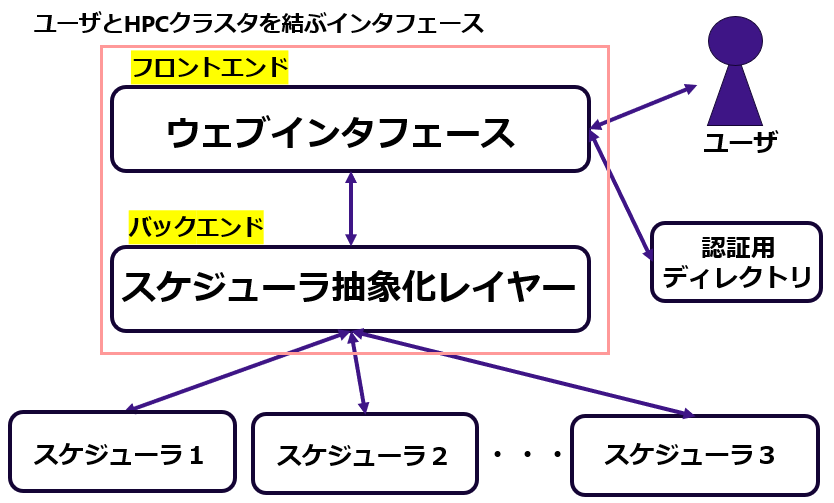
\includegraphics[width=75mm]{./fig/proposed_method.png}
  \caption{提案手法}
  \label{fig1}
\end{figure}

\vspace{3\baselineskip}
\section{ウェブインタフェースを介したHPCシステム利用環境}
ウェブ機能とスケジューラ抽象化機能をそれぞれ独立に実装し,連携させることでウェブインタフェースを介して様々なシステムを統一的に利用できる環境を実現する.そのために,ウェブ機能の基盤としてOOD,スケジューラ抽象化機能の基盤としてPSI/J\cite{citation_6}と呼ばれるPythonライブラリを利用し,両者を組み合わせることで提案手法を実装する.\par
本研究では,東北大学のスーパーコンピュータ「AOBA」で運用されているジョブスケジューラ(NEC Network Queuing System V, NQSV)がOODに対応していないという事実に着目して,NQSVをスケジューラ抽象化機能側に実装することと,それをウェブ機能側から利用できることを検証する.
実行環境として,OOD用のホストサーバとスーパーコンピュータAOBAを模したHPCクラスタを考える.HPCクラスタでは,AOBAと同様にNQSVがジョブスケジューラとして利用されている.OODはログイン時に必要な認証用のディレクトリであるActive Directory(AD)と連携する.\par
はじめに,スケジューラ抽象化機能のNQSV対応を考える.PSI/Jは,ジョブの情報を格納するJobクラスとジョブの投入や削除などのメソッドをスケジューラごとに再定義しているJobExecutorクラスにより構成されている.本研究では新たにNQSV用のJobExecutorクラスを作成し,ジョブの投入,削除,ジョブの状態確認を行うための3つのメソッドを実装する.PSI/Jが対応している他のスケジューラ(Slurm, PBS Pro, LSF, Flux, Cobalt)はジョブの終了後にジョブの状態(COMPLETED,CANCELED,FAILED)をコマンドの出力結果から確認できる.しかし,NQSVではジョブの終了後にCOMPLETED,CANCELED,FAILEDの状態を確認できない.そのため,NQSVに対応するためには,ジョブの投入,ジョブの削除,および待機中のジョブの存在確認に基づいてジョブの状態をPSI/J側で把握する必要がある.この機能を実現するため,本研究の実装ではジョブが投入された後にジョブキューからジョブが無くなった際に,そのジョブの状態をCOMPLETEDに変更する.また,ジョブが削除された際には,そのジョブの状態をCANCELEDに変更する.それ以外にジョブキューの状態をコマンドを用いて定期的に確認し,出力結果に応じてQUEUEDあるいはACTIVEという状態にする.このようにPSI/J自身がジョブの状態を管理することにより,さらに広い範囲のジョブスケジューラに対応することができることから,ジョブスケジューラ抽象化機能の汎用性を高めることができたといえる.\par
続いて,ウェブ機能側であるOOD側からスケジューラ機能を用いることを考える.実装における問題点として,OODがRubyで実装されていることに対して,PSI/JはPythonで実装されているという点が挙げられる.そのため,Rubyスクリプト上でPythonライブラリを使用する必要がある.本実装ではPSI/Jを経由する際のオーバヘッドが小さく,単純な実装であるため,PSI/Jを用いたジョブの管理のためのPythonスクリプトをシェルを経由してRubyスクリプト上で直接実行する.この実装により,ウェブ機能としてOODを用い,スケジューラ抽象化機能であるPSI/Jを経由して,指定したスケジューラにジョブの投入や削除を行うことができる.また,PSI/Jを仲介することで,OODが未対応であったNQSVでのジョブ管理をOOD上から操作することを実現している.\par
図\ref{fig4}はOOD上でジョブを作成して投入と削除を行う「Job Composer」の画面である.ジョブを作成する際にクラスタを「psij」に設定することで,PSI/Jを経由してSlurmクラスタやNQSVクラスタなど任意のHPCシステムにジョブを投入できていることが確認できた.\par

\begin{figure}[tb]
  \centering
  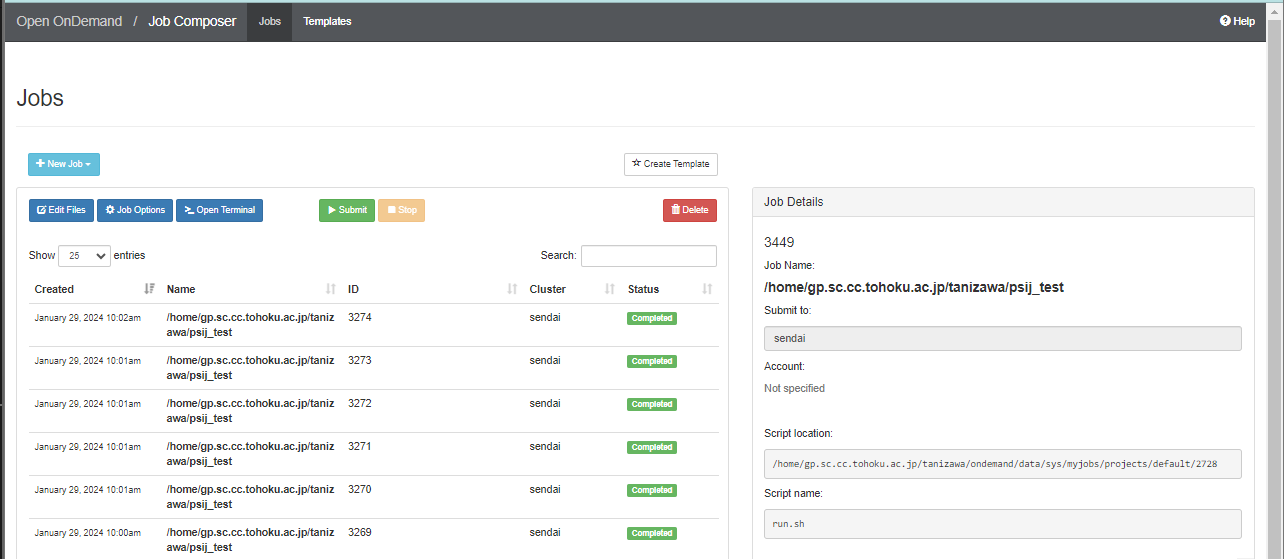
\includegraphics[width=75mm]{./fig/jobcomposer.png}
  \caption{Job Composerの画面}
  \label{fig4}
\end{figure}

\vspace{3\baselineskip}
\section{評価と考察}
インタフェースをウェブ機能とスケジューラ抽象化機能に分けたことによって両者の連携時のオーバヘッドの発生が懸念されるため,その影響を定量的に評価する.本実装においては,OODがシェルを介してPSI/JのPythonスクリプトを実行するため,そのオーバヘッドによる影響を評価する.評価には,Seleniumと呼ばれるウェブページの自動制御ライブラリを用いる.ローカルホストから別ホストのOODのポータルサイトにアクセスして,Job Composer画面でジョブの作成と投入を行う.ジョブの作成を開始した時刻から,そのジョブの実行を完了した時刻までを計測し,ジョブのターンアラウンドタイムとする.ジョブの投入を1~10回連続で行い,そのターンアラウンドタイムを計測してPSI/Jを経由する場合と経由しない場合を比較した結果を図\ref{fig2}および図\ref{fig3}に示す。\par

\begin{figure}[tb]
  \centering
  \hspace{-11mm}
  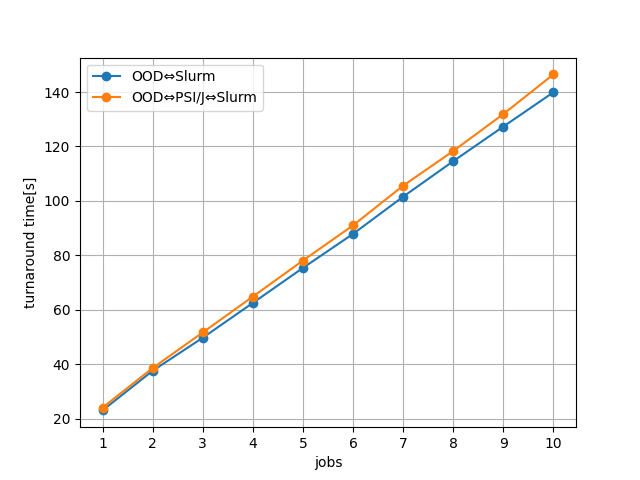
\includegraphics[width=85mm, height=55mm]{./fig/ave_1-20.png}
  \vspace{-10pt}
  \caption{実行時オーバーヘッドの比較}
  \label{fig2}
\end{figure}

\begin{figure}[tb]
  \centering
  \hspace{-11mm}
  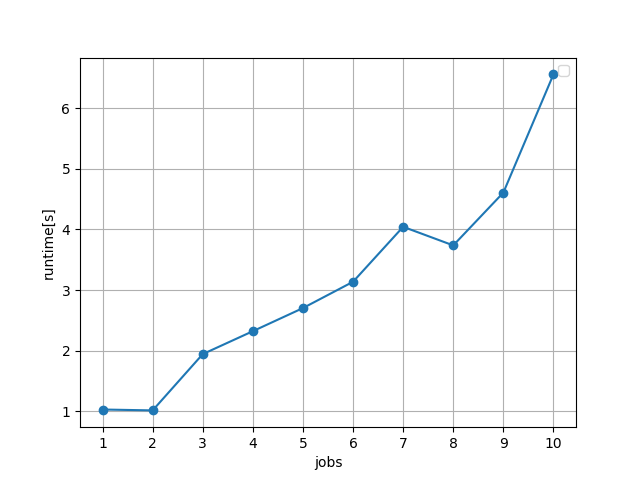
\includegraphics[width=85mm, height=55mm]{./fig/ave_diff_1-20.png}
  \vspace{-10pt}
  \caption{実行時オーバーヘッドの差}
  \label{fig3}
\end{figure}

ターンアラウンドタイムはそれぞれ合計20回計測され,その平均値が図\ref{fig2}および図\ref{fig3}に示されている.横軸は連続して投入したジョブの数を示す.図\ref{fig2}の縦軸はジョブのターンアラウンドタイムを示し,図\ref{fig3}の縦軸はジョブのターンアラウンドタイムの差を示す.図\ref{fig2}からPSI/Jを経由した提案手法の方がわずかにターンアラウンドタイムが大きいことがわかり,どちらの場合も連続投入したジョブの数に線形比例して増加していることがわかる.また図\ref{fig3}から,ジョブの連続投入回数が多くなればなるほど両者の実行時オーバヘッドの差が大きくなっていることがわかる.\par
次に,ジョブを1~100回連続投入した際の実行時オーバヘッドを比較する.図\ref{fig5}は,ジョブの連続投入数を10回ずつ増やしたときのターンアラウンドタイムの比較を示している.1~10回の連続投入の場合と同じく,PSI/Jを経由した場合の方がわずかにターンアラウンドタイムが大きくなっており,連続投入するジョブ数を大きくしても極端にオーバヘッドに差が出ることはないということがわかった.ジョブの連続投入回数に依らず,PSI/Jを経由した場合のオーバヘッドは,PSI/Jを経由しない場合のターンアラウンドタイムの5%以内に収まり,提案手法によって生じるオーバヘッドは十分無視できるといえる.\par

\begin{figure}[tb]
  \centering
  \hspace{-11mm}
  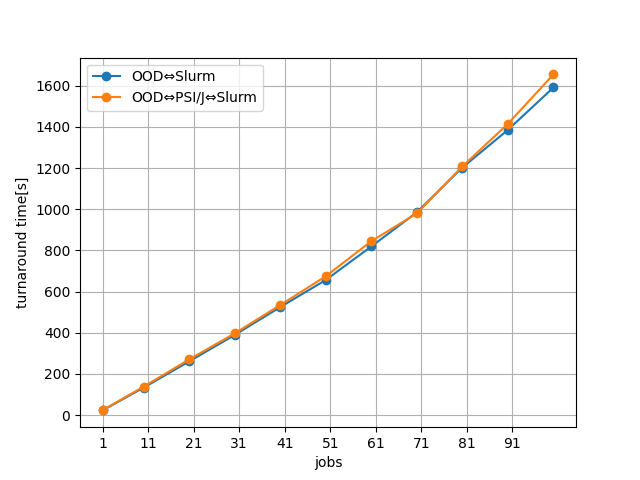
\includegraphics[width=85mm, height=55mm]{./fig/100jobs.png}
  \vspace{-10pt}
  \caption{ジョブ数を増加した際のオーバヘッドの比較}
  \label{fig5}
\end{figure}

\vspace{3\baselineskip}
\section{結論}
本研究では,HPCシステムの利用難易度の高さやスケジューラ多様化に伴うシステムの保守性の問題という背景のもと,HPC利用者の支援という目的で,HPCシステムの簡易な利用環境と充分なシステムの保守性を合わせ持つウェブインタフェースの実装について考えた.この実現のために,ウェブ機能とスケジューラ抽象化機能を分離し,それぞれ独立に保守管理する手法を提案した.\par
提案手法では,OODをインタフェースとしてPSI/Jを介してジョブの投入と削除を実現している.実行時オーバヘッドを測定して比較することで,OODとPSI/Jの連携のために生じる実行時オーバヘッドは十分に小さいことが明らかになった.また,PSI/J側でNQSVに対応することによってOODからNQSVを利用可能となり,ウェブ機能とジョブスケジューラ抽象化機能の分離の実現可能性と有用性を示すことができた.\par
現在,OODがジョブの一旦停止(hold)と再開(release)の操作も提供しているのに対して,PSI/Jではそれらの操作に対応していない.これらの操作に必要な両者の連携を設計して実装していくことで,より多様なジョブスケジューラやその使い方に対応可能となると期待される.その検討は今後の課題である.\par

\vspace{3\baselineskip}
\bibliographystyle{junsrt}
\bibliography{refer}

\end{document}